%!TEX root = ../thesis.tex

\section{Preliminaries}
\fxinnote{Lead in paragraph}
\fxinnote{define notations and concepts in one go}
\fxinnote{state results at and of this section}

\mypar{Paths}
  A path $\P$ is a sequence of vertices such that every two consecutive vertices are connected with each other. The first and last vertex of the path are its \emph{extreme} vertices while the rest are \emph{interior} vertices of this path. The \emph{length} of a path is the number of edges used to connect the vertices. That, is one less then the number of vertices. All paths are \emph{simple}, that is, no vertex occurs twice in the path except the extreme vertices.

\mypar{Cycles}
  We call a cycle of length $k$  a \emph{$k$-cycle}. A \emph{triangle} is cycle of length $3$ (i.e. a $3$-cycle).
  By Jordan's curve theorem a cycle splits the plane into two parts, one bounded and one unbounded. We will call the bounded part the \emph{interior} of this cycle and the unbounded part the \emph{exterior} of this cycle.
  We call a cycle \emph{separating} if there are vertices in both its interior and exterior.
  An \emph{interior edge} of a cycle is then an edge contained in the interior of the cycle.
  An \emph{interior path} is a path connecting two distinct vertices off the cycle and whose edges are interior edges.

\mypar{Path notations}
  We denote the vertices of a path $\P$ by $p_1 \ldots p_k$.
  With $\rev{P}$ we denote the \emph{reversed path} $p_k \ldots p_1$. We use $\oplus$ to denote the \emph{concatenation} of paths. That is, given a second path $\Q$ with vertices $q_1 \ldots q_l$ and $p_k = q_1$ the path $\P \oplus \Q$ consists of $p_1 \ldots p_{k-1} q_1 q_2 \ldots q_l$.
  Recall that a cycle is simply a path starting and ending at the same vertex. Hence if we have two  internally disjoint paths $\P, \Q$ from $s$ to $t$ then $\P \oplus \rev{\Q}$ is a cycle.
  Furthermore we use a vertical bar to denote the \emph{restriction} of a path to a certain set of vertices. So $\P|_{p_i, p_j}$ with $i<j$ is the subpath of $\P$ with vertices $p_i \ldots p_j$.

\mypar{Chords}
  \fxinnote{Move to relevant place}
  A \emph{chord} of a path is an edge that connects two vertices in this path, but is not part of the path. A path without chords is \emph{chordfree}.
  A \emph{k-chord} is a path $\Q$ of length $k$ that connects two non-subsequent vertices $p_i, p_j$ of $\P$ such that $\P \cap \Q = \braces{p_i, p_j}$.
  Since a cycle is a special type of path the same definitions also apply to them.
  Note that $\P|_{v_i, v_j} \oplus \rev{\Q}$ is a cycle. The ($k$-)chord $\Q$ is \emph{separating} if this cycle is separating.

\mypar{Rotations}
  \fxinnote{Move to relevant place}
  We fix an embedding for all graphs in this thesis. In this embedding the \emph{rotation} at a vertex $v$ is the clockwise order of the edges incident to $v$. We will identify these edges with their other endpoints.
  Two vertices $x, y$ are said to be \emph{consecutive} in the rotation at $v$ when the edges $vx$ and $vy$ are consecutive.
  Given a path $\P$ and a interior vertex $p_i$. A neighbor $v \nin \P$ of $p_i$ lies on the \emph{left} of $\P$ if it lies in the interval from $p_{i-1}$ to $p_{i+1}$ in the clockwise rotation at $p_{i}$. Otherwise $v$ lies in the interval from $p_{i+1}$ to $p_{i-1}$ in the rotation clockwise at $p_i$. In this case $v$ lies on the \emph{right} of $\P$.
  We will use the same notion of left and right for edges. That is, an edge $e\nin P$ adjacent to $p_i$ lies to left or right if its other end point lies to the left or right, respectively.



    \subsection{Adjacent vertices and chords}
    \fxnote{introduce where this gets relevant}
    We call a vertex \emph{$\pS$-adjacent} when it is adjacent to $\pS$ in the current corner assignment. In the same way we call a chord or $2$-chord \emph{$\pE$-bound}, \emph{$\pW$-bound} or \emph{polebound} when it is adjacent to $\pE$, $\pW$ or any pole,  respectively.

    \subsubsection{Fans}
    We introduce some more concepts to describe the interior of a blue (or red) face. Every interior edge of this face goes from one fence to the other (otherwise its start or end vertex would violate the interior vertex condition).\fxnote{This could be a useful result in the section about cycles and their interiors.} To better understand the structure of such a strip we will describe the edges from $\spl(F)$ to $\mrg(F)$ .

    Let $u_0 , u_1, \ldots u_n$ be the vertices of the upper boundary path of $F$ and $v_0, v_1, \ldots, v_m$ the vertices of the bottom boundary path. That is $u_0=v_0 = \spl(F)$ and $u_n = v_m = \mrg(F)$. Since our graph is a triangulation $u_1v_1$ must be an edge. For the second edge in the face we have two options $u_1v_2$ or $u_2v_1$, otherwise this edge and the previous one would not form a triangle. This principle holds for every subsequent edge, we can either increase the index of the upper boundary path or the index of the bottom boundary path. In other words, this face is a so-called \emph{triangle strip}.

    We call a maximal sequence of at least two edges increasing the index on the bottom boundary path (and thus keeping the index on the upper path fixed) a \emph{Bottom-fan} or simply \emph{B-fan} and a maximal sequence of at least two edges increasing the index on the upper boundary path is called a \emph{Top-fan} or just \emph{T-fan}. \fxnote*{Q What's wrong here?}{The \emph{size} of such a fan is the number of edges contained in the sequence}. By the definition of a fan it has size of at least $2$.
    We use \emph{fans} to refer to both these \emph{types} of fans (i.e. T- and B-fans).
    We call a fan of size $3$ or larger a \emph{large fan} and a fan of size $2$ a \emph{small fan}.

    In a strip we alternately encounter B- and T-fans. Since if we would have two adjacent fans of the same type we would just have a single larger fan of that type.
    In Figure \ref{fig:uni:fans} we see a strip consisting of subsequently a B-fan of size $3$, a T-fan of size 2, a B-fan of size $2$, a T-fan of size $6$, a B-fan of size $3$ and a T-fan of size $3$.

    \begin{figure}[h]
      \centering
      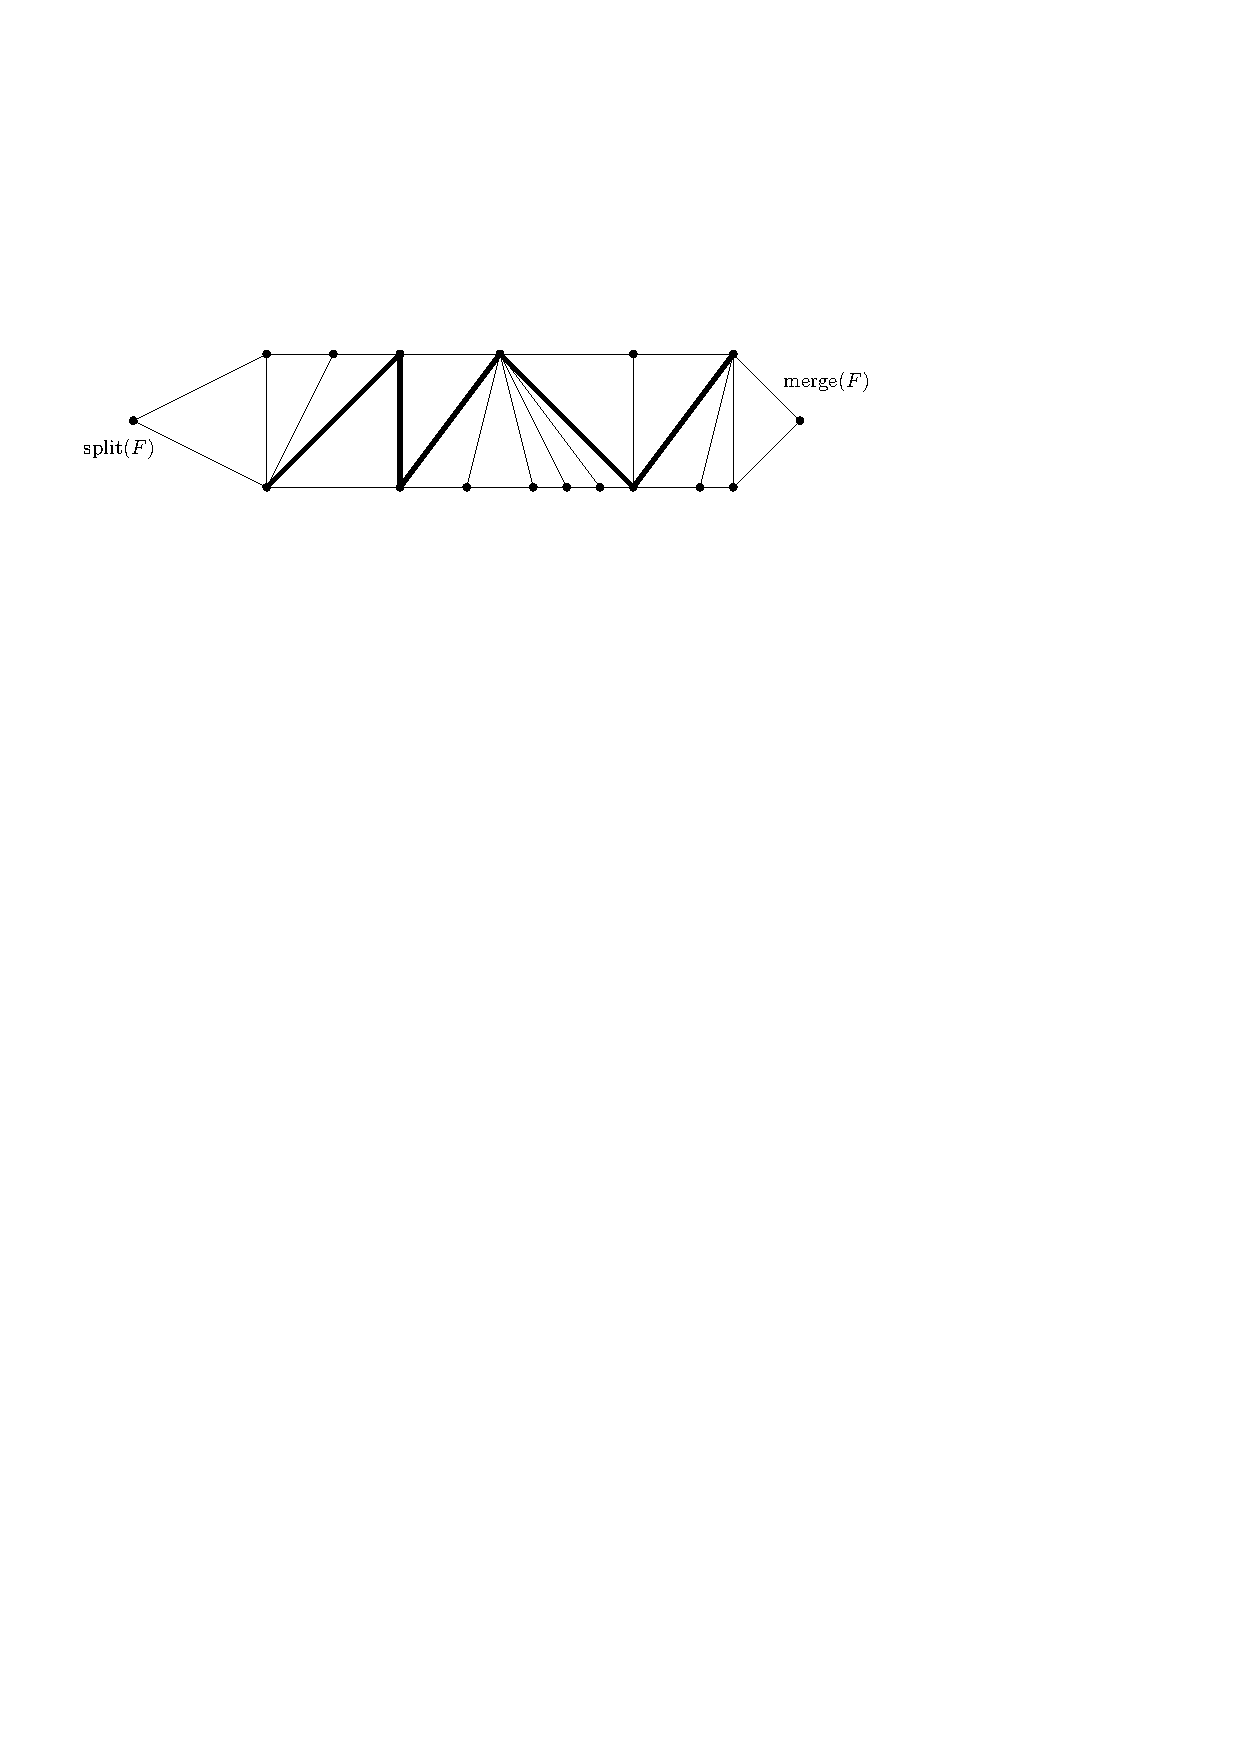
\includegraphics[scale=.9]{rectangularDuals/img/fans}
      \caption{}
      \label{fig:uni:fans}
    \end{figure}


   We introduce some more terminology for fans: \emph{outer edges}, \emph{fan handles} and the \emph{rim} as can be seen in Figure \ref{fig:rect:fanTerms}. The \emph{fan handle} $v$ is the vertex shared by all edges in the fan. Let $F$ be the induced subgraph of vertices adjacent to the edges in the fan. $F$ contains no edges not belonging to the triangle strip since these would lead to separating 3-cycles. The \emph{rim} is the path given by $F\sm{v}$.
   \fxnote{Q is this definition of Rim more clear or still unclear?}
   \fxnote*{Do we use this}{The \emph{outer rim} are the two extreme edges of this path and} the \emph{outer edges} are the edges between the fan handles and the extreme vertices of the \emph{rim}.

   \begin{figure}[h]
     \centering
     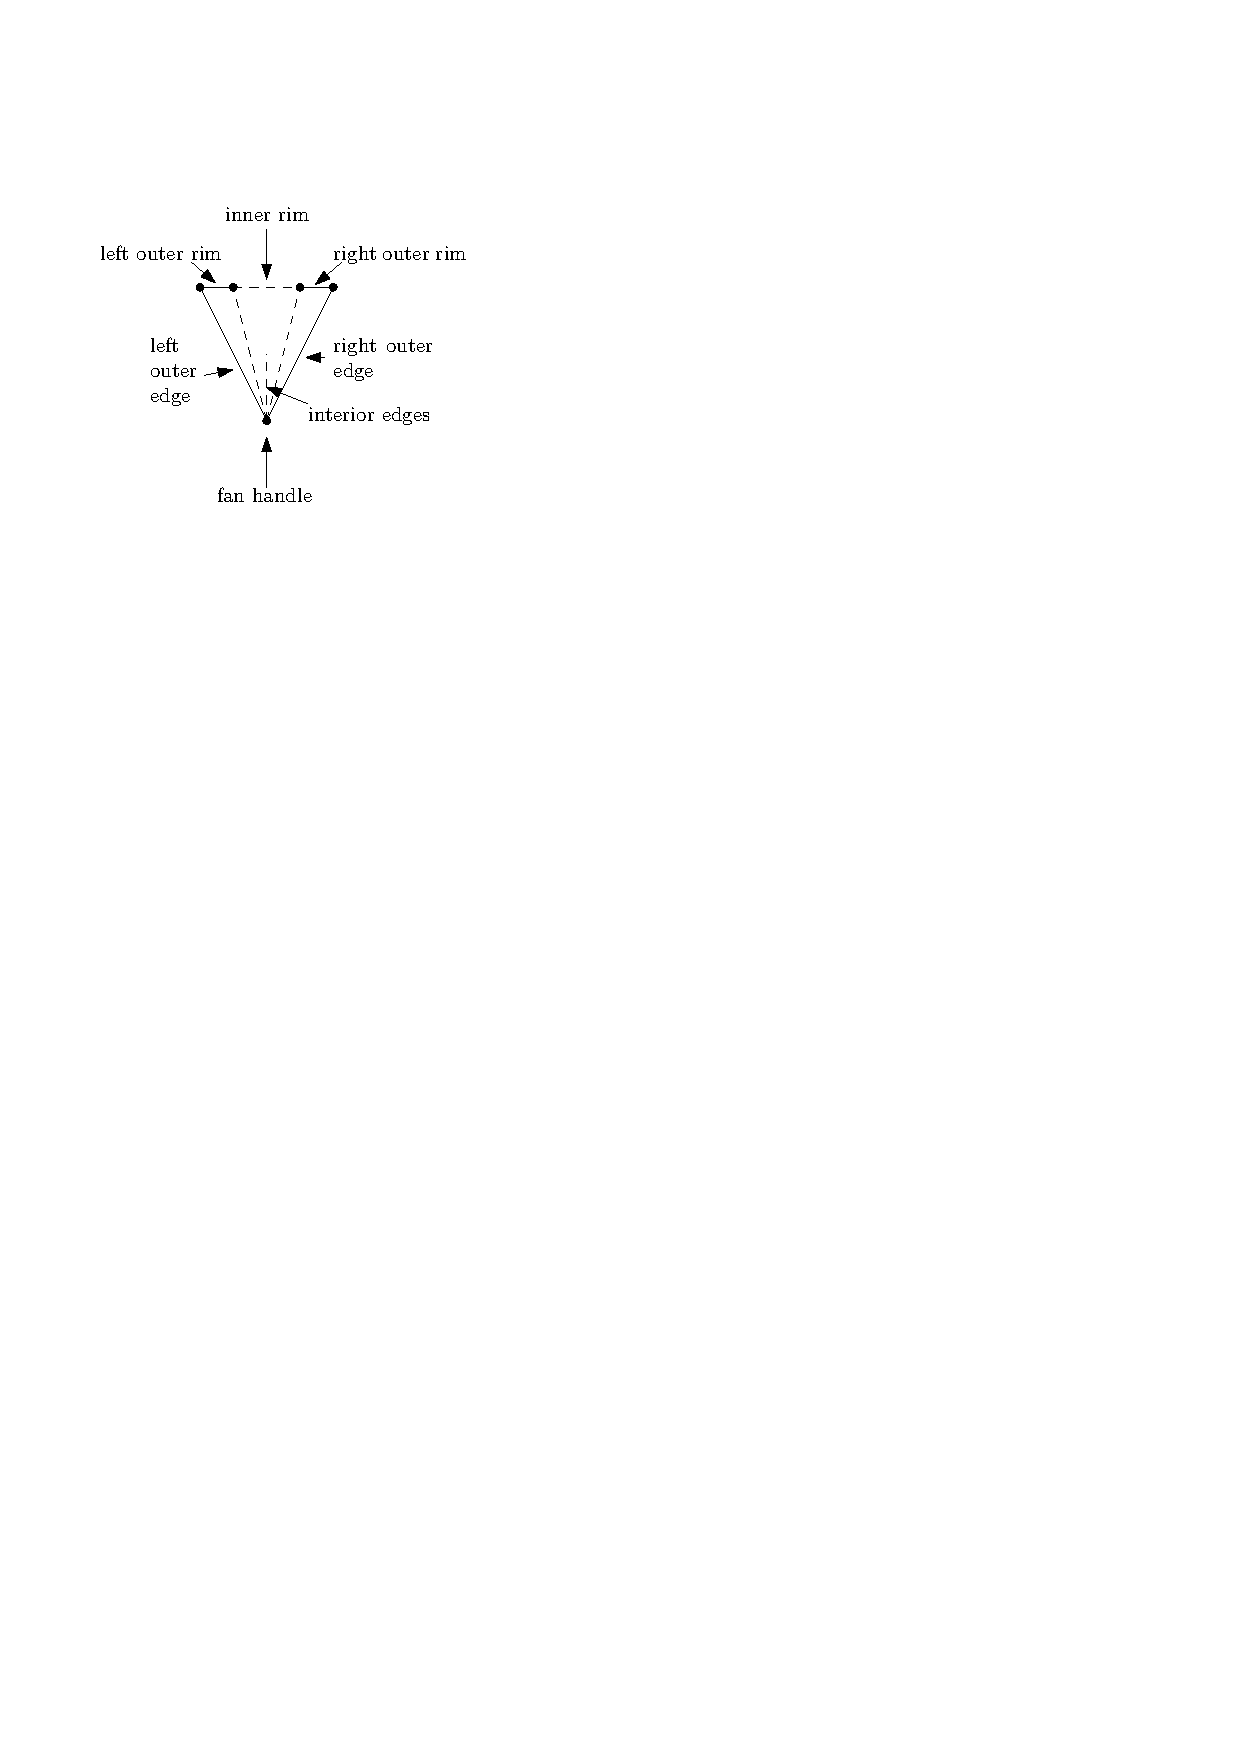
\includegraphics[scale=1]{rectangularDuals/img/fanterms}
     \caption{}
     \label{fig:rect:fanTerms}
   \end{figure}
